

\begin{figure*}
\centering
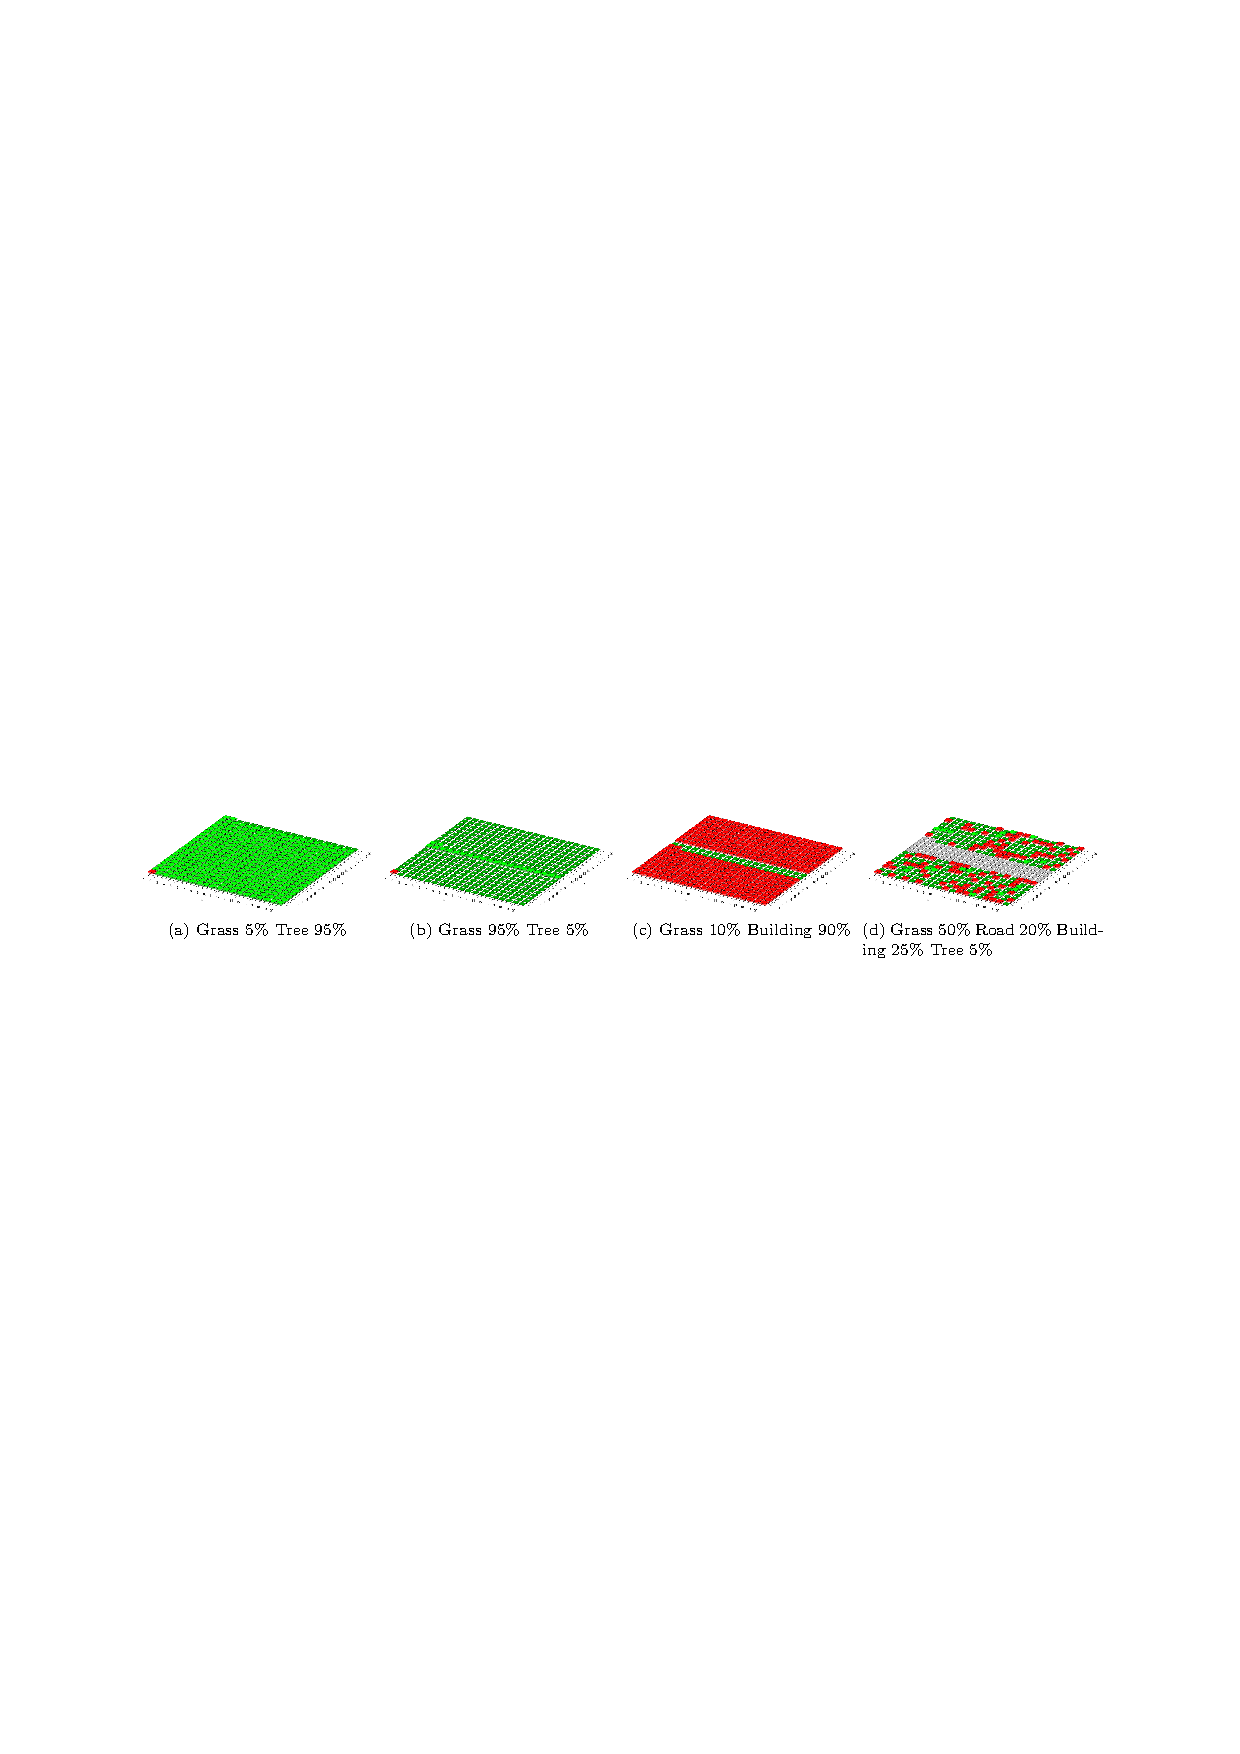
\includegraphics[page=1,trim={70 380 60 390},clip,scale=0.65]{Figures/Figures.pdf}
\caption{\bf Creation of VTUF-3D scenarios for 9814 variations of parameters across representative ranges in Melbourne.}
 \label{fig:scenarios}
\end{figure*} 


\begin{figure*}
\centering
\includegraphics[page=2,trim={75 240 60 240},clip,scale=0.35]{Figures/PresentationImages.pdf}
\caption{\bf Example VTUF-3D results of UTCI at ground surface levels for a Melbourne scenario.}
 \label{fig:vtufresults}
\end{figure*} 


\begin{figure*}
\centering
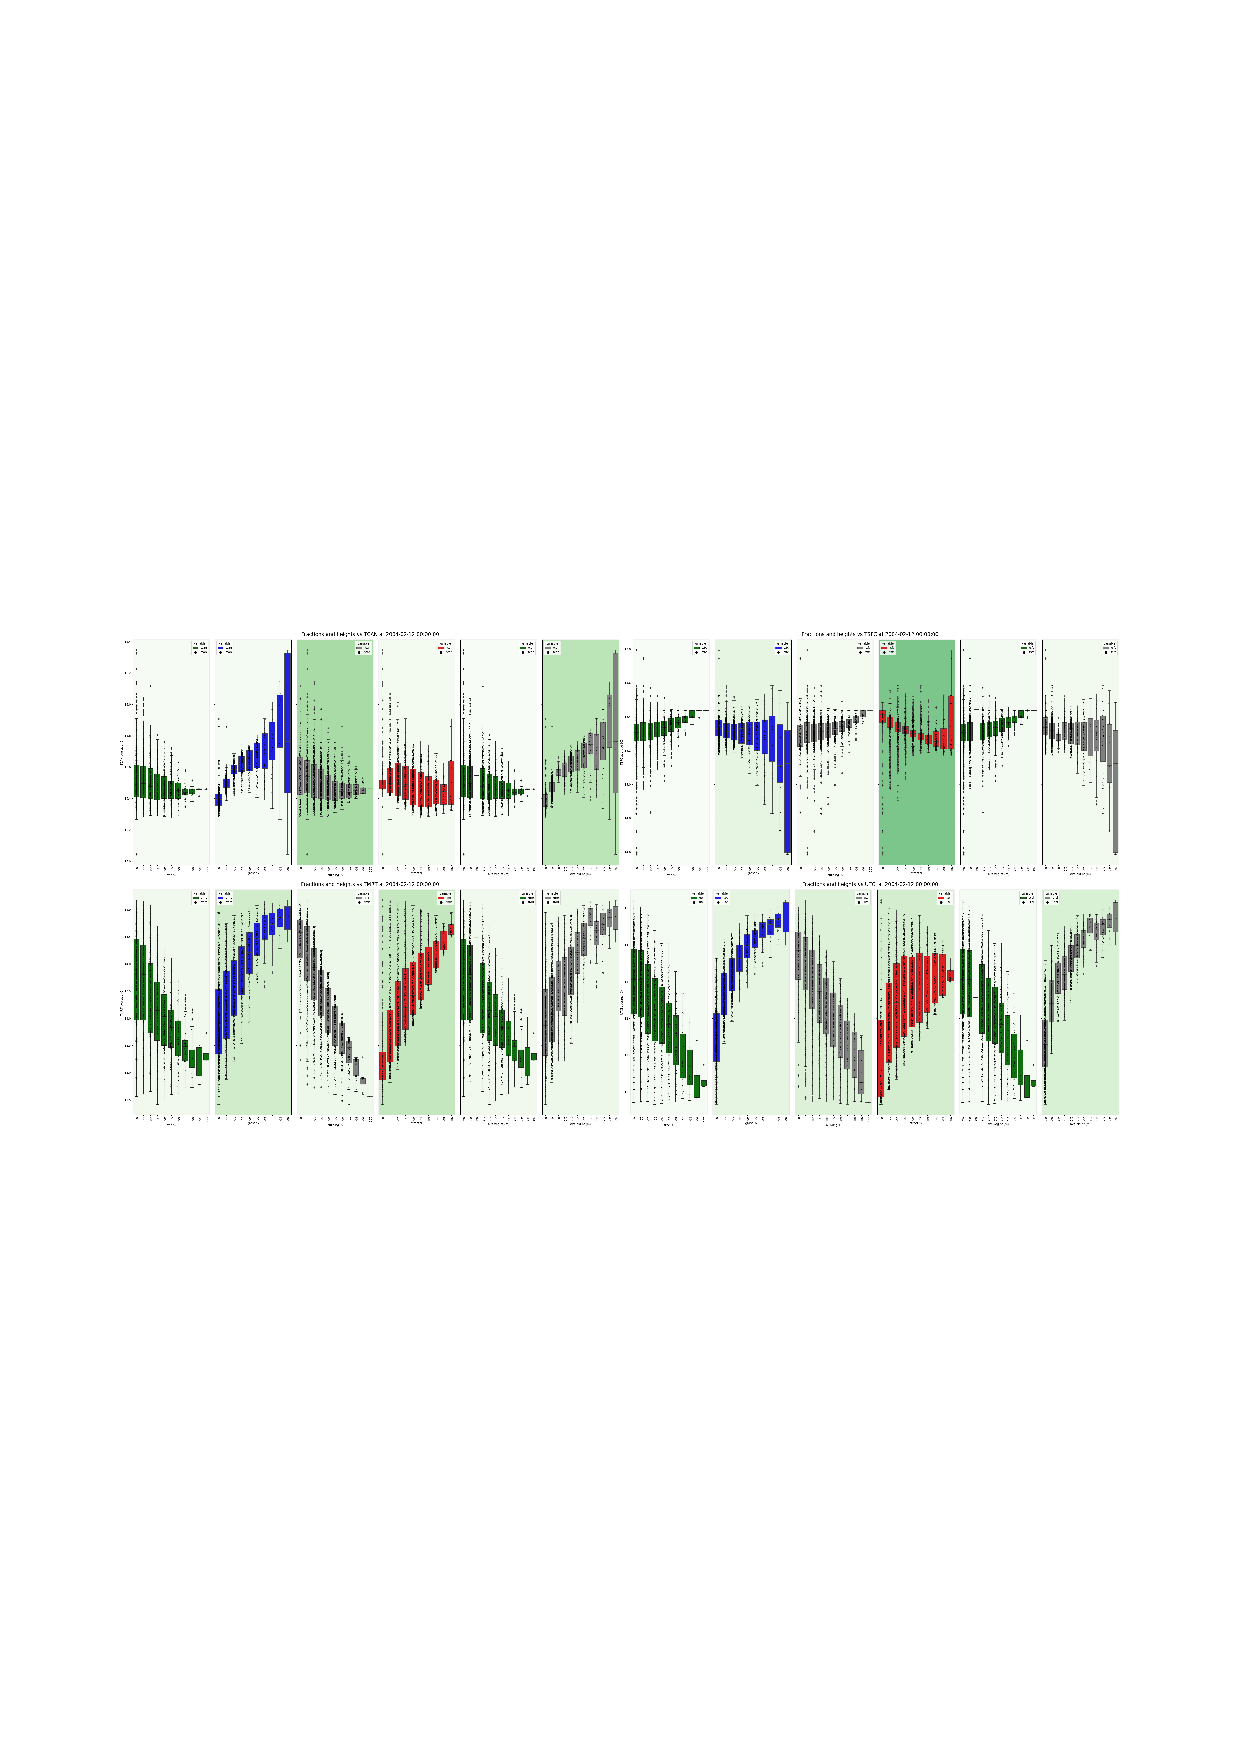
\includegraphics[page=1,trim={60 300 50 300},clip,scale=1.0]{Figures/Figures2.pdf}
\caption{\bf Surface fractions percentages and average heights vs. temperatures (\gls{tcan}, \gls{tsfc}, \gls{tmrt}, and \gls{utci}) for February 12, 2004, 12am. Feature importance for each temperature type is indicated by the green background tinting.}
 \label{fig:box0}
\end{figure*} 

\begin{figure*}
\centering
\includegraphics[page=2,trim={60 300 50 300},clip,scale=1.0]{Figures/Figures2.pdf}
\caption{\bf Surface fractions percentages and average heights vs. temperatures (\gls{tcan}, \gls{tsfc}, \gls{tmrt}, and \gls{utci}) for February 12, 2004, 5am. Feature importance for each temperature type is indicated by the green background tinting.}
 \label{fig:box5}
\end{figure*} 

\begin{figure*}
\centering
\includegraphics[page=3,trim={60 300 50 300},clip,scale=1.0]{Figures/Figures2.pdf}
\caption{\bf Surface fractions percentages and average heights vs. temperatures (\gls{tcan}, \gls{tsfc}, \gls{tmrt}, and \gls{utci}) for February 12, 2004, 2pm. Feature importance for each temperature type is indicated by the green background tinting.}
 \label{fig:box14}
\end{figure*} 


\begin{figure*}
\centering

\includegraphics[page=34,trim={124 250 120 250},clip,scale=0.8]{Figures/Figures4.pdf}
\caption{\bf Surface fractions percentages and average heights vs. temperatures (\gls{tcan} and \gls{utci}) for February 12, 2004, 12am. Feature importance for each temperature type is indicated by the green background tinting.}
 \label{fig:box0a}
\end{figure*} 

\begin{figure*}
\centering
\includegraphics[page=35,trim={124 250 120 250},clip,scale=0.8]{Figures/Figures4.pdf}
\caption{\bf Surface fractions percentages and average heights vs. temperatures (\gls{tcan} and \gls{utci}) for February 12, 2004, 5am. Feature importance for each temperature type is indicated by the green background tinting.}
 \label{fig:box5a}
\end{figure*} 

\begin{figure*}
\centering
\includegraphics[page=36,trim={124 250 120 250},clip,scale=0.8]{Figures/Figures4.pdf}
\caption{\bf Surface fractions percentages and average heights vs. temperatures (\gls{tcan} and \gls{utci}) for February 12, 2004, 2pm. Feature importance for each temperature type is indicated by the green background tinting.}
 \label{fig:box14a}
\end{figure*} 





\begin{figure*}
\centering
{\tiny a)}\includegraphics[page=36,trim={55 275 50 295},clip,scale=0.45]{Figures/Figures3.pdf}
{\tiny b)}\includegraphics[page=37,trim={55 275 50 295},clip,scale=0.45]{Figures/Figures3.pdf}\\
{\tiny c)}\includegraphics[page=38,trim={55 275 50 295},clip,scale=0.45]{Figures/Figures3.pdf}
{\tiny d)}\includegraphics[page=39,trim={55 275 50 295},clip,scale=0.45]{Figures/Figures3.pdf}
\caption{\bf Feature importance in a) \gls{tcan}, b) \gls{tmrt}, c) \gls{tsfc}, and d) \gls{utci} for the four surface fractions of streets, buildings, trees, and grass and the two average heights of vegetation and buildings across 11-12 February 2004. }
\label{fig:featimpttcan}
\label{fig:featimpttmrt}
\label{fig:featimpttsfc}
\label{fig:featimptutci}
\end{figure*}


\begin{figure*}
\centering
\includegraphics[page=15,trim={92 245 92 245},clip,scale=0.95]{Figures/Figures4.pdf}
\caption{\bf Mean \gls{tcan} outcomes clustered by 10\% surface fraction ranges of a) grass, b) streets, c) trees, and d) buildings and e) average vegetation and f) average building heights clustered by 0.8m increases over a diurnal cycle of 14 February 2004.  }
 \label{fig:tcanday}
\end{figure*}

\begin{figure*}
\centering
\includegraphics[page=16,trim={92 245 92 245},clip,scale=0.95]{Figures/Figures4.pdf}
\caption{\bf Mean \gls{tmrt} outcomes clustered by 10\% surface fraction ranges of a) grass, b) streets, c) trees, and d) buildings and e) average vegetation and f) average building heights clustered by 0.8m increases over a diurnal cycle of 14 February 2004. }
 \label{fig:tmrtday}
\end{figure*}

\begin{figure*}
\centering
\includegraphics[page=17,trim={92 245 92 245},clip,scale=0.95]{Figures/Figures4.pdf}
\caption{\bf Mean \gls{tsfc} outcomes clustered by 10\% surface fraction ranges of a) grass, b) streets, c) trees, and d) buildings and e) average vegetation and f) average building heights clustered by 0.8m increases over a diurnal cycle of 14 February 2004. }
 \label{fig:tsfcday}
\end{figure*}

\begin{figure*}
\centering
\includegraphics[page=18,trim={92 245 92 245},clip,scale=0.95]{Figures/Figures4.pdf}
\caption{\bf Mean \gls{utci} outcomes clustered by 10\% surface fraction ranges of a) grass, b) streets, c) trees, and d) buildings and e) average vegetation and f) average building heights clustered by 0.8m increases over a diurnal cycle of 14 February 2004. }
 \label{fig:utciday}
\end{figure*}





\begin{figure*}
\centering
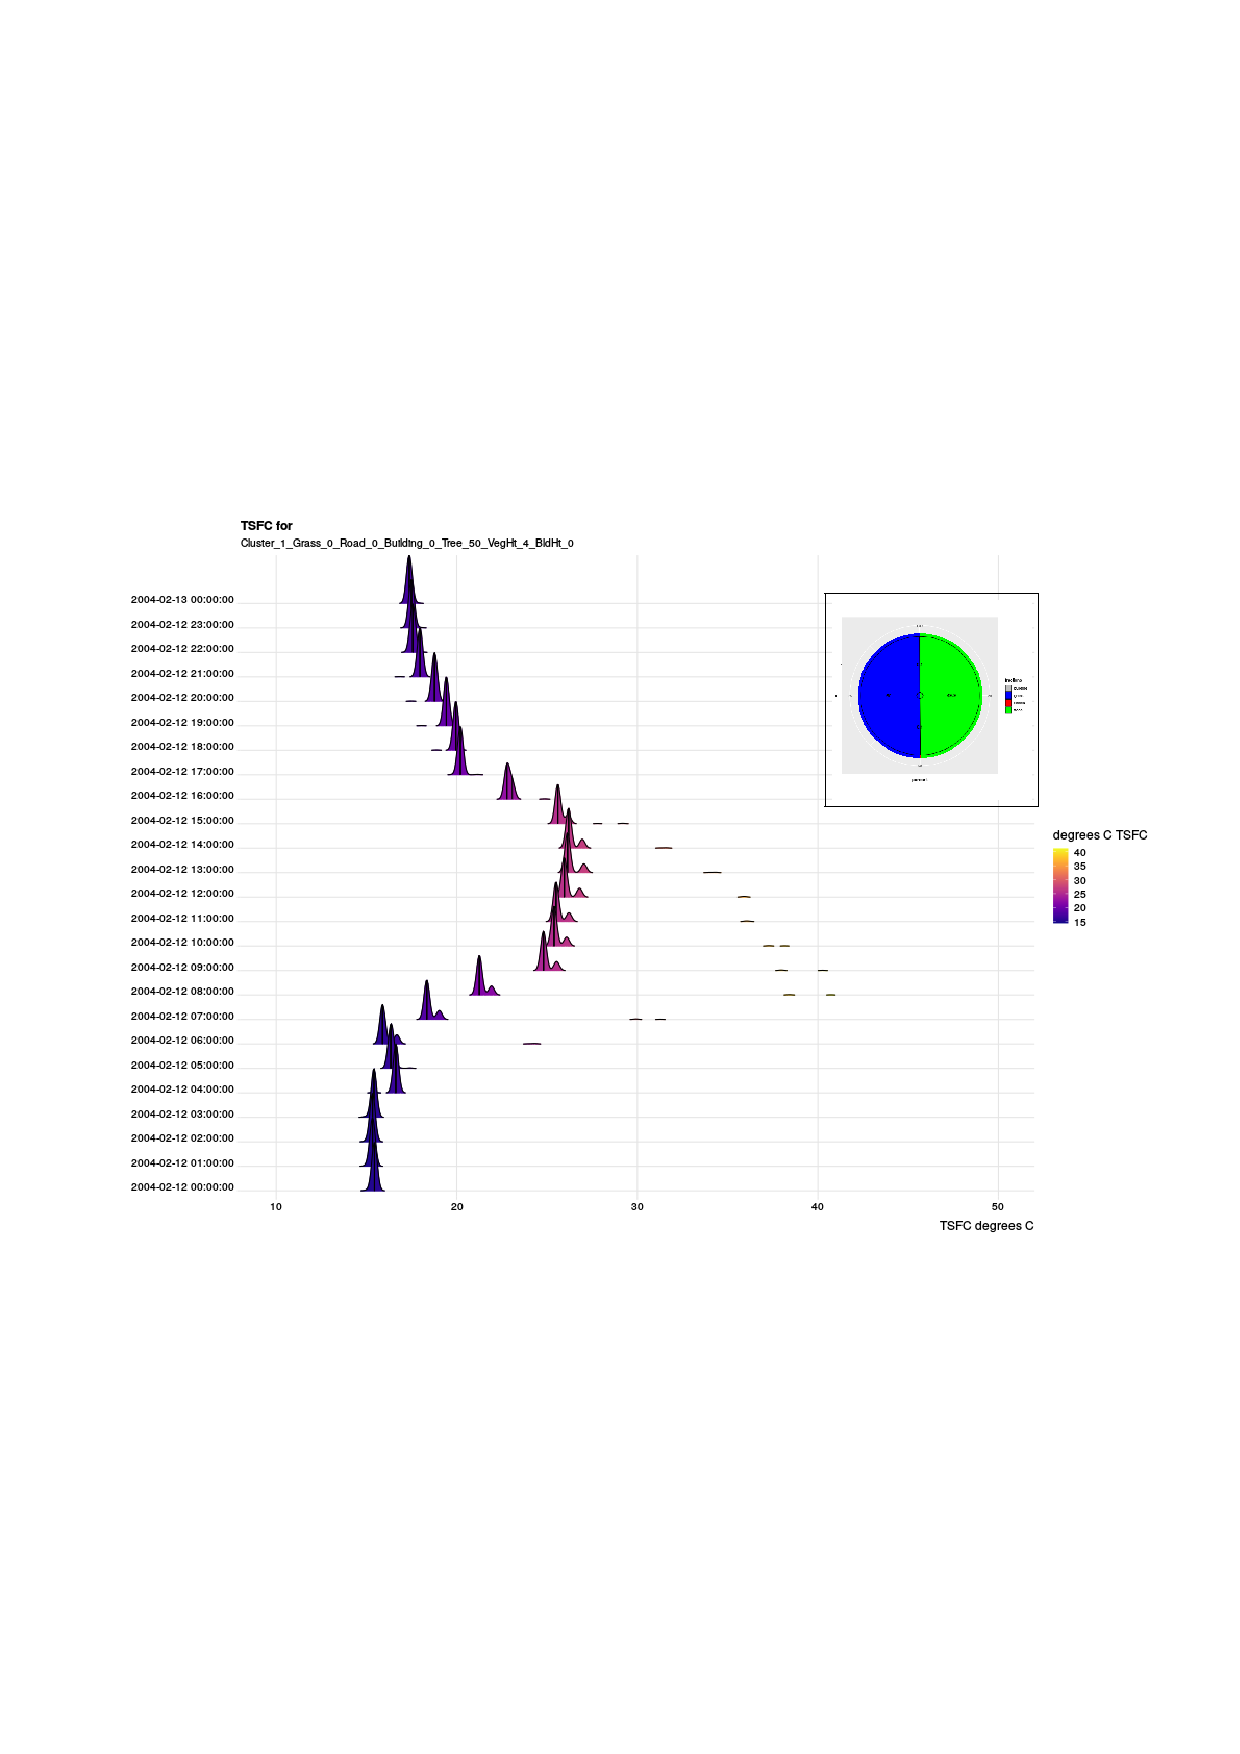
\includegraphics[page=1,trim={60 250 63 266},clip,scale=0.5]{Figures/Figures3.pdf}
\caption{\bf Distribution of \gls{tsfc} across February 12, 2004 for scenario 50\% grass, 49.99\% trees, 0.01\% road, 0\% building, average vegetation height of 4m, and average building height of 0m. Insert shows percent fractions of surface types.}
 \label{fig:dist1}
\end{figure*}

\begin{figure*}
\centering
\includegraphics[page=3,trim={60 250 63 266},clip,scale=0.5]{Figures/Figures3.pdf}
\caption{\bf Distribution of \gls{tsfc} across February 12, 2004 for scenario 29\% grass, 70\% trees, 1\% road, 0\% building, average vegetation height of 0.5m, and average building height of 0m. Insert shows percent fractions of surface types.}
 \label{fig:dist3}
\end{figure*}

\begin{figure*}
\centering
\includegraphics[page=5,trim={60 250 63 266},clip,scale=0.5]{Figures/Figures3.pdf}
\caption{\bf Distribution of \gls{tsfc} across February 12, 2004 for scenario 89\% grass, 0\% trees, 8\% road, 3\% building, average vegetation height of 0m, and average building height of 5m. Insert shows percent fractions of surface types.}
 \label{fig:dist5}
\end{figure*}

\begin{figure*}
\centering
\includegraphics[page=2,trim={60 250 63 266},clip,scale=0.5]{Figures/Figures3.pdf}
\caption{\bf Distribution of \gls{tsfc} across February 12, 2004 for scenario 19\% grass, 10\% trees, 30\% road, 40\% building, average vegetation height of 2m, and average building height of 6m. Insert shows percent fractions of surface types.}
 \label{fig:dist2}
\end{figure*}

\begin{figure*}
\centering
\includegraphics[page=4,trim={60 250 63 266},clip,scale=0.5]{Figures/Figures3.pdf}
\caption{\bf Distribution of \gls{tsfc} across February 12, 2004 for scenario 19\% grass, 10\% trees, 20\% road, 50\% building, average vegetation height of 1m, and average building height of 30m. Insert shows percent fractions of surface types.}
 \label{fig:dist4}
\end{figure*}

\begin{figure*}
\centering
\includegraphics[page=6,trim={60 250 63 266},clip,scale=0.5]{Figures/Figures3.pdf}
\caption{\bf Distribution of \gls{tsfc} across February 12, 2004 for scenario 40\% grass, 10\% trees, 20\% road, 30\% building, average vegetation height of 2m, and average building height of 14m. Insert shows percent fractions of surface types.}
 \label{fig:dist6}
\end{figure*}

\begin{figure*}
\centering
\includegraphics[page=7,trim={60 250 63 266},clip,scale=0.5]{Figures/Figures3.pdf}
\caption{\bf Distribution of \gls{tsfc} across February 12, 2004 for scenario 19\% grass, 20\% trees, 21\% road, 40\% building, average vegetation height of 1m, and average building height of 9m. Insert shows percent fractions of surface types.}
 \label{fig:dist7}
\end{figure*}




\begin{figure*}
\centering
a)\includegraphics[page=14,trim={155 270 147 328},clip,scale=0.75]{Figures/Figures2.pdf}
b)\includegraphics[page=15,trim={155 270 141 328},clip,scale=0.75]{Figures/Figures2.pdf}
\caption{\bf a) \gls{tcan} and b) \gls{tsfc} heatmaps on February 12, 2004 at 2pm generated by matching the closest matching parameters of surface fractions and average heights for each 100$\times$100m location in Melbourne from 9814 modelled scenario results.  }
 \label{fig:TaMelb} \label{fig:TsfcMelb}
\end{figure*}


\begin{figure*}
\centering
\includegraphics[page=19,trim={92 245 92 245},clip,scale=0.95]{Figures/Figures4.pdf}
\caption{\bf Surface fractions of a) grass, b) trees, c) buildings, and d) streets across Melbourne.}
 \label{fig:melfracs}
\end{figure*}



\begin{figure*}
\centering
a)\includegraphics[page=14,trim={220 255 75 315},clip,scale=0.70]{Figures/Figures3.pdf}
b)\includegraphics[page=20,trim={180 255 95 315},clip,scale=0.70]{Figures/Figures3.pdf}\\
c)\includegraphics[page=26,trim={94 328 295 338},clip,scale=0.60]{Figures/Figures3.pdf}
d)\includegraphics[page=26,trim={59 353 380 345},clip,scale=0.70]{Figures/Figures4.pdf}
e)\includegraphics[page=22,trim={43 325 470 325},clip,scale=0.60]{Figures/Figures4.pdf}
\caption{\bf a) Landsat 8 land surface temperature in degrees kelvin captured 10am December 11, 2018. Local conditions of air temperature on this day were minimum and maximum of 22 and 26\SI{}{\degreeCelsius}. b) Differences in surface temperatures (modelled \gls{tsfc} minus observed Landsat 8 LST) on February 12, 2004 at 10am generated by matching the closest matching parameters of surface fractions and average heights for each 100$\times$100m location in Melbourne from 9814 modelled scenario results. Histograms of temperature distributions of c) modelled \gls{tsfc} (February 12, 2004 at 10am) and d) observed Landsat 8 LST (December 11, 2018 at 10am). e) Correlations between surface fraction amounts and differences in temperatures (as shown in b).}
 \label{fig:Melb_TSFC12_85}
\end{figure*}


\begin{figure*}
\centering
a)\includegraphics[page=15,trim={220 255 75 315},clip,scale=0.70]{Figures/Figures3.pdf}
b)\includegraphics[page=21,trim={180 255 95 315},clip,scale=0.70]{Figures/Figures3.pdf}\\
c)\includegraphics[page=27,trim={94 328 295 338},clip,scale=0.60]{Figures/Figures3.pdf}
d)\includegraphics[page=25,trim={59 353 380 345},clip,scale=0.70]{Figures/Figures4.pdf}
e)\includegraphics[page=31,trim={43 325 470 325},clip,scale=0.60]{Figures/Figures4.pdf}
\caption{\bf a) Landsat 8 land surface temperature in degrees kelvin captured 10am December 27, 2018. Local conditions of air temperature on this day were minimum and maximum of 15 and 39\SI{}{\degreeCelsius}. b) Differences in surface temperatures (modelled \gls{tsfc} minus observed Landsat 8 LST) on February 14, 2004 at 10am generated by matching the closest matching parameters of surface fractions and average heights for each 100$\times$100m location in Melbourne from 9814 modelled scenario results. Histograms of temperature distributions of c) modelled \gls{tsfc} (February 12, 2004 at 10am) and d) observed Landsat 8 LST (December 27, 2018 at 10am). e) Correlations between surface fraction amounts and differences in temperatures (as shown in b).}
 \label{fig:Melb_TSFC14_85}
\end{figure*}





\begin{figure*}
\centering
a)\includegraphics[page=17,trim={155 255 141 328},clip,scale=0.75]{Figures/Figures2.pdf}
b)\includegraphics[page=18,trim={155 255 147 328},clip,scale=0.75]{Figures/Figures2.pdf}
\caption{\bf a) \gls{tmrt} and b) \gls{utci} heatmaps on February 12, 2004 at 2pm generated by matching the closest matching parameters of surface fractions and average heights for each 100$\times$100m location in Melbourne from 9814 modelled scenario results.  }
 \label{fig:TmrtMelb}
 \label{fig:utciMelb}
\end{figure*}



\begin{figure*}
\centering
a)\includegraphics[page=19,trim={200 300 175 350},clip,scale=1.0]{Figures/Figures2.pdf}
b)\includegraphics[page=20,trim={200 300 170 350},clip,scale=1.0]{Figures/Figures2.pdf}
\caption{\bf a) \gls{tcan} and b) \gls{tsfc} heatmaps on February 12, 2004 at 2pm generated by matching the closest matching parameters of surface fractions and average heights for each 100$\times$100m location in Sydney from 9814 modelled scenario results.  }
 \label{fig:TaSyd}
\end{figure*}

\begin{figure*}
\centering
\includegraphics[page=20,trim={92 245 92 245},clip,scale=0.95]{Figures/Figures4.pdf}
\caption{\bf Surface fractions of a) grass, b) trees, c) buildings, and d) streets across Sydney.}
 \label{fig:sydfracs}
\end{figure*}




%16 Sydney-Landsat-LST-11-03-2019  %//  11/03/2019	22	26
\begin{figure*} 
\centering
a)\includegraphics[page=16,trim={210 265 115 315},clip,scale=0.75]{Figures/Figures3.pdf}
b)\includegraphics[page=22,trim={210 265 110 315},clip,scale=0.75]{Figures/Figures3.pdf}\\
c)\includegraphics[page=28,trim={94 328 295 338},clip,scale=0.60]{Figures/Figures3.pdf}
d)\includegraphics[page=28,trim={59 353 380 345},clip,scale=0.70]{Figures/Figures4.pdf}
e)\includegraphics[page=23,trim={43 325 470 325},clip,scale=0.60]{Figures/Figures4.pdf}
\caption{\bf b) Landsat 8 land surface temperature in degrees kelvin captured 10am March 11, 2019. Local conditions of air temperature on this day were minimum and maximum of 22 and 26\SI{}{\degreeCelsius}. c) Differences in surface temperatures (modelled \gls{tsfc} minus observed Landsat 8 LST) on February 12, 2004 at 10am generated by matching the closest matching parameters of surface fractions and average heights for each 100$\times$100m location in Sydney from 9814 modelled scenario results. Histograms of temperature distributions of c) modelled \gls{tsfc} (February 12, 2004 at 10am) and d) observed Landsat 8 LST (March 11, 2019 at 10am). e) Correlations between surface fraction amounts and differences in temperatures (as shown in b). }
 \label{fig:Sydney-Landsat-LST-11-03-2019}
 \label{fig:Sydney_TSFC12_85}
\end{figure*}





%17 Sydney-Landsat-LST-19-01-2018  %//  19/01/2018	18	31
\begin{figure*}  
\centering
a)\includegraphics[page=17,trim={200 265 115 315},clip,scale=0.75]{Figures/Figures3.pdf}
b)\includegraphics[page=23,trim={200 265 115 315},clip,scale=0.75]{Figures/Figures3.pdf}\\
c)\includegraphics[page=29,trim={94 328 295 338},clip,scale=0.60]{Figures/Figures3.pdf}
d)\includegraphics[page=27,trim={59 353 380 345},clip,scale=0.70]{Figures/Figures4.pdf}
e)\includegraphics[page=23,trim={43 325 470 325},clip,scale=0.60]{Figures/Figures4.pdf}
\caption{\bf a) Landsat 8 land surface temperature in degrees kelvin captured 10am 19 January 2018. Local conditions of air temperature on this day were minimum and maximum of 18 and 31\SI{}{\degreeCelsius}. b) Differences in surface temperatures (modelled \gls{tsfc} minus observed Landsat 8 LST) on February 12, 2004 at 10am generated by matching the closest matching parameters of surface fractions and average heights for each 100$\times$100m location in Sydney from 9814 modelled scenario results. Histograms of temperature distributions of c) modelled \gls{tsfc} (February 14, 2004 at 10am) and d) observed Landsat 8 LST (January 19, 2018 at 10am). e) Correlations between surface fraction amounts and differences in temperatures (as shown in b).}
 \label{fig:Sydney-Landsat-LST-19-01-2018}
 \label{fig:Sydney-Landsat-TSFC-LST-19-01-2018}
 \label{fig:Sydney_TSFC14_85}
\end{figure*}



\begin{figure*}
\centering
a)\includegraphics[page=22,trim={200 300 170 350},clip,scale=0.95]{Figures/Figures2.pdf}
b)\includegraphics[page=23,trim={200 300 170 350},clip,scale=0.95]{Figures/Figures2.pdf}
\caption{\bf a) Mean radiant temperature and b) \gls{utci}  heatmaps on February 12, 2004 at 2pm generated by matching the closest matching parameters of surface fractions and average heights for each 100$\times$100m location in Sydney from 9814 modelled scenario results.  }
 \label{fig:utciSyd}\label{fig:TmrtSyd}
\end{figure*}





\begin{figure*}
\centering
a)\includegraphics[page=24,trim={200 300 180 350},clip,scale=1.0]{Figures/Figures2.pdf}
b)\includegraphics[page=25,trim={200 300 180 350},clip,scale=1.0]{Figures/Figures2.pdf}
\caption{\bf a) Air temperature and b) surface temperature heatmaps on February 12, 2004 at 2pm generated by matching the closest matching parameters of surface fractions and average heights for each 100$\times$100m location in Perth from 9814 modelled scenario results.  }
 \label{fig:TaPerth}\label{fig:TsfcPerth}
\end{figure*}

\begin{figure*}
\centering
\includegraphics[page=21,trim={92 245 92 245},clip,scale=0.95]{Figures/Figures4.pdf}
\caption{\bf Surface fractions of a) grass, b) trees, c) buildings, and d) streets across Perth.}
 \label{fig:perthfracs}
\end{figure*}


%18 Perth-Landsat-LST-29-03-2019  % //  29/03/2019	13	27
\begin{figure*}  
\centering
a)\includegraphics[page=18,trim={220 260 137 321},clip,scale=0.75]{Figures/Figures3.pdf}
b)\includegraphics[page=24,trim={170 260 137 321},clip,scale=0.75]{Figures/Figures3.pdf}
c)\includegraphics[page=30,trim={94 328 295 338},clip,scale=0.60]{Figures/Figures3.pdf}
d)\includegraphics[page=29,trim={59 353 380 345},clip,scale=0.70]{Figures/Figures4.pdf}
e)\includegraphics[page=24,trim={43 325 470 325},clip,scale=0.60]{Figures/Figures4.pdf}
%\caption{\bf Perth-Landsat-LST-29-03-2019  29/03/2019	13	27}
\caption{\bf a) Landsat 8 land surface temperature in degrees kelvin captured 10am March 29, 2019. Local conditions of air temperature on this day were minimum and maximum of 13 and 27\SI{}{\degreeCelsius}. b) Differences in surface temperatures (modelled \gls{tsfc} minus observed Landsat 8 LST) on February 12, 2004 at 10am generated by matching the closest matching parameters of surface fractions and average heights for each 100$\times$100m location in Perth from 9814 modelled scenario results. Histograms of temperature distributions of c) modelled \gls{tsfc} (February 14, 2004 at 10am) and d) observed Landsat 8 LST (March 29, 2019 at 10am). e) Correlations between surface fraction amounts and differences in temperatures (as shown in b). }
 \label{fig:Perth-Landsat-LST-29-03-2019}
 \label{fig:Perth-Landsat-TSFC-LST-29-03-2019}
 \label{fig:Perth_TSFC12_85}
\end{figure*}






%19 Perth-Landsat-LST-25-02-2019   %  //  25/02/2019	19	37
\begin{figure*} 
\centering
a)\includegraphics[page=19,trim={220 260 137 321},clip,scale=0.75]{Figures/Figures3.pdf}
b)\includegraphics[page=25,trim={160 260 137 321},clip,scale=0.75]{Figures/Figures3.pdf}\\
c)\includegraphics[page=31,trim={94 328 295 338},clip,scale=0.60]{Figures/Figures3.pdf}
d)\includegraphics[page=30,trim={59 353 380 345},clip,scale=0.70]{Figures/Figures4.pdf}
e)\includegraphics[page=33,trim={43 325 470 325},clip,scale=0.60]{Figures/Figures4.pdf}
\caption{\bf a) Landsat 8 land surface temperature in degrees kelvin captured 10am 25 February 2019. Local conditions of air temperature on this day were minimum and maximum of 19 and 37\SI{}{\degreeCelsius}. b) Differences in surface temperatures (modelled \gls{tsfc} minus observed Landsat 8DSAT8 LST) on February 12, 2004 at 10am generated by matching the closest matching parameters of surface fractions and average heights for each 100$\times$100m location in Perth from 9814 modelled scenario results. Histograms of temperature distributions of c) modelled \gls{tsfc} (February 14, 2004 at 10am) and d) observed Landsat 8 LST (February 25, 2019 at 10am). e) Correlations between surface fraction amounts and differences in temperatures (as shown in b). }
 \label{fig:Perth-Landsat-LST-25-02-2019}
 \label{fig:Perth-Landsat-TSFC-LST-25-02-2019}
 \label{fig:Perth_TSFC14_85}
\end{figure*}


